\documentclass[]{article}
\usepackage[T1]{fontenc}
\usepackage[utf8]{inputenc}
\usepackage{amsmath}
\usepackage{listings}
\usepackage{graphicx} 
\usepackage{hyperref}

%opening
\title{Distributed Battleships - Manual}
\author{Annika Laumets, Andre Tättar, Viktoria Plemakova, Sander Tars}

\begin{document}
\lstset{language=Python}  

\maketitle

\section*{Setup process and dependencies}

Repository: \url{https://github.com/crypotex/distributed-battleship}\\

Firstly, the (middleware) dependencies are pika python library and RabbitMQ. They have to be installed. Pika can be installed using \textit{pip}. If using Linux, RabbitMQ can be installed using \textit{apt-get}.

\noindent To run the application, first server needs to be run. To do this, from the command line run the file "server.py" from the \textit{server} directory. That should set up the server.

\noindent Once the server is running, client user interfaces can be opened by running "gui.py" from the command line. The file "gui.py" is located in the \textit{client} directory. 
\newpage

\section*{User interface manual}
The user interface is explained by the following screenshots and their descriptions.


\begin{figure}[!hbt]
	\centering
	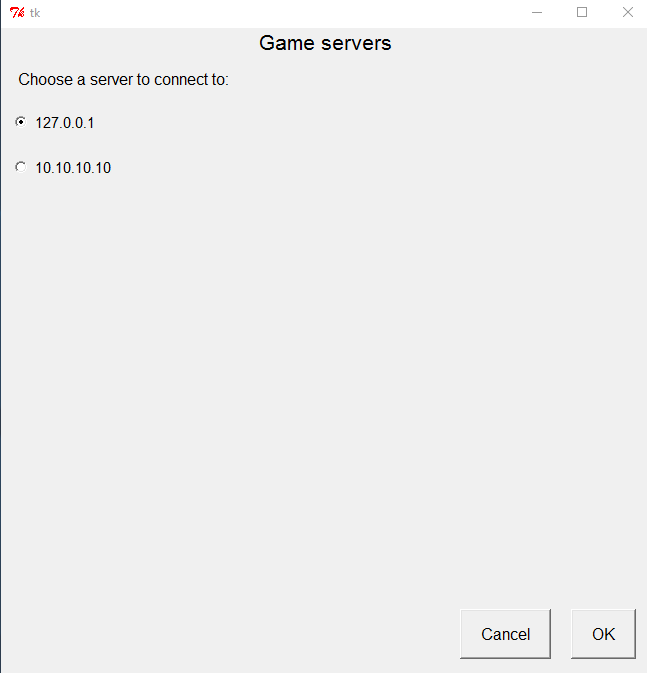
\includegraphics[width=0.8\textwidth]{OpenPage.png}
	\caption{Opening page of the user interface. A list of available servers is displayed for connecting. OK button proceeds to the name choosing. Cancel button closes the application.}
	\label{fig:Openpage}
\end{figure}

\begin{figure}[!hbt]
	\centering
	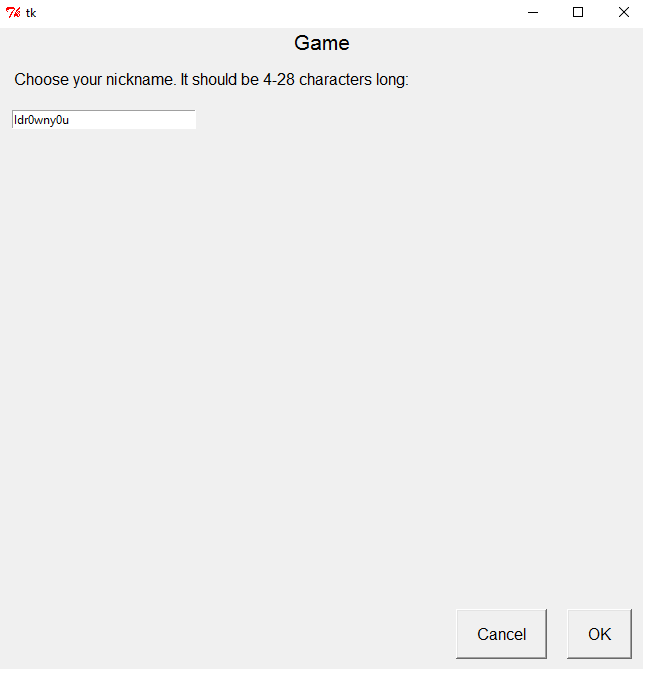
\includegraphics[width=0.8\textwidth]{NickPage.png}
	\caption{Nickname choosing page for user. A nickname can be entered in the text box. OK button sends the nickname and proceeds to the game choosing if nickname has been approved by the server. Cancel button goes back to server choosing view. If the nickname is unsuitable, a pop-up is presented.}
	\label{fig:Nickpage}
\end{figure}

\begin{figure}[!hbt]
	\centering
	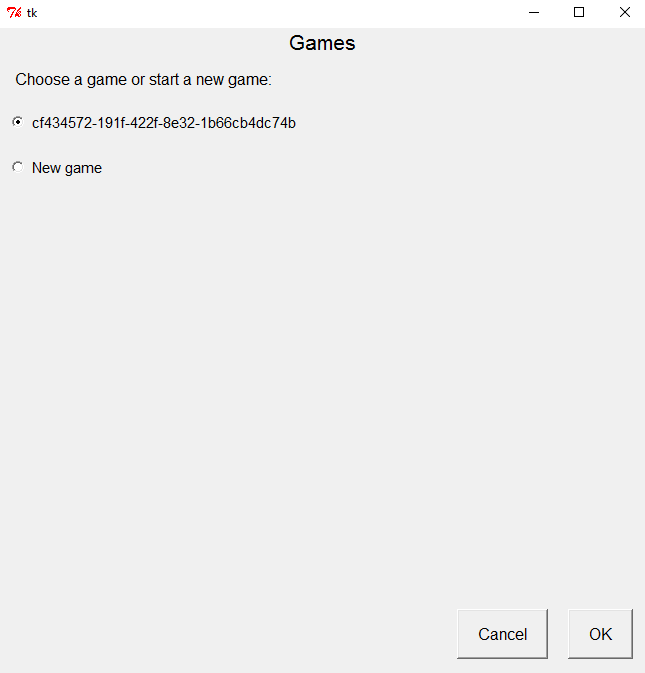
\includegraphics[width=0.8\textwidth]{ChooseGame.png}
	\caption{Game can be chosen from a displayed list or a new game can be created. OK proceeds to the next view, Cancel returns to the server choosing view.}
	\label{fig:Choosegame}
\end{figure}

\begin{figure}[!hbt]
	\centering
	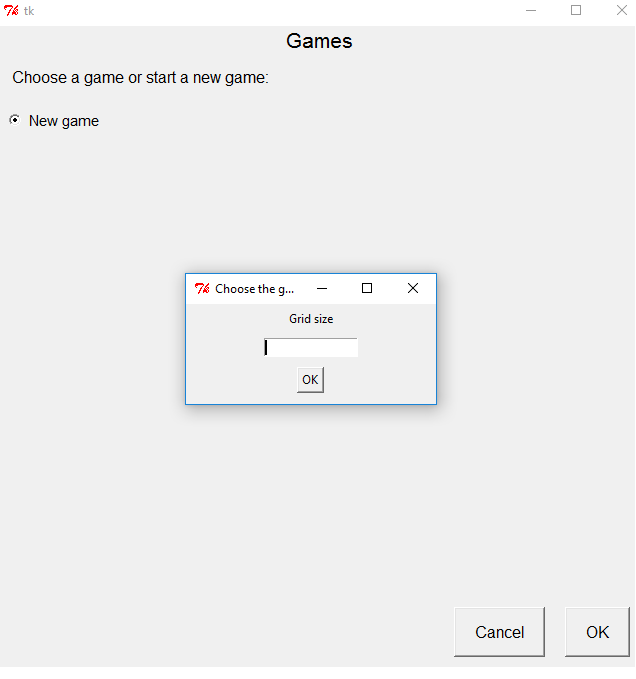
\includegraphics[width=0.8\textwidth]{GridSize.png}
	\caption{In case a new game is created, user is prompted with a pop-up to choose the grid size. OK button proceeds to the ship placement view.}
	\label{fig:Gridsize}
\end{figure}

\begin{figure}[!hbt]
	\centering
	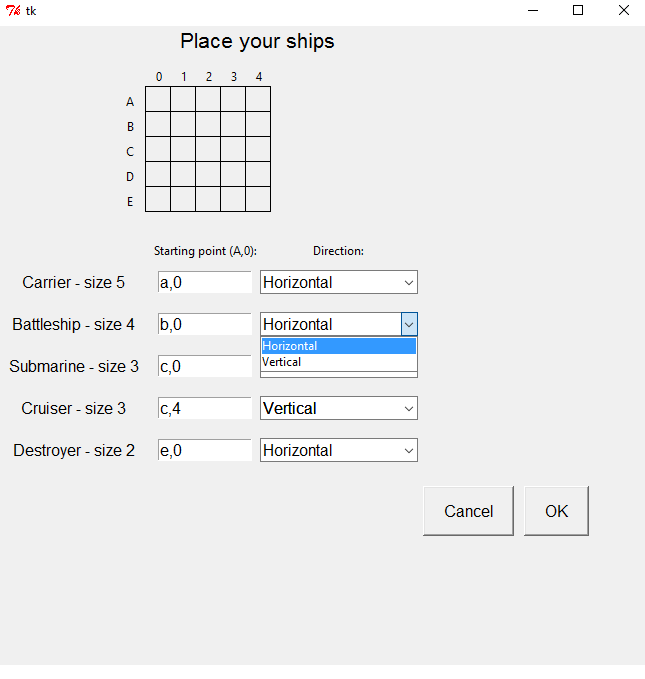
\includegraphics[width=0.8\textwidth]{ShipPlace.png}
	\caption{Ship placement view of the UI. User can choose the "root" place of the ship by typing it in the textbox and the direction of the ships by choosing from the dropdown menu. OK button proceeds to the game "lobby", Cancel button returns to the game choosing view.}
	\label{fig:ShipPlace}
\end{figure}

\begin{figure}[!hbt]
	\centering
	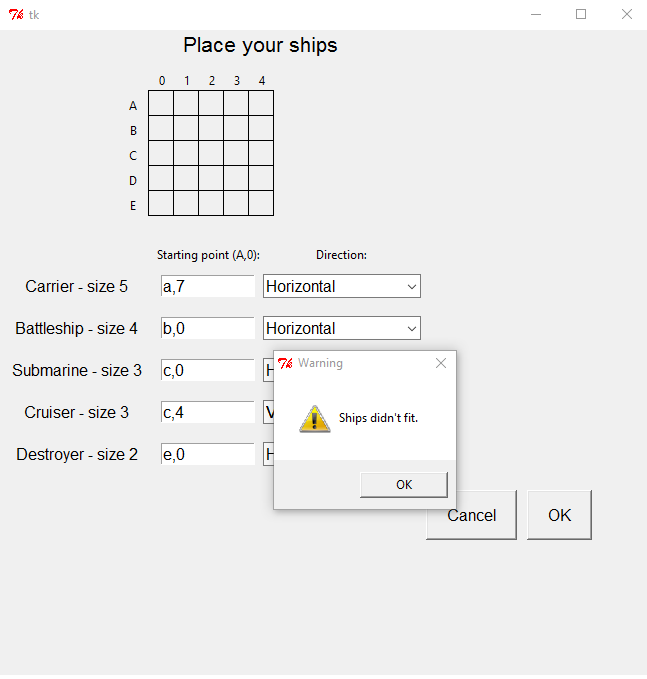
\includegraphics[width=0.8\textwidth]{ShipUnfit.png}
	\caption{In case ship placement is unfit, user is notified with a pop-up.}
	\label{fig:ShipUnfit}
\end{figure}

\begin{figure}[!hbt]
	\centering
	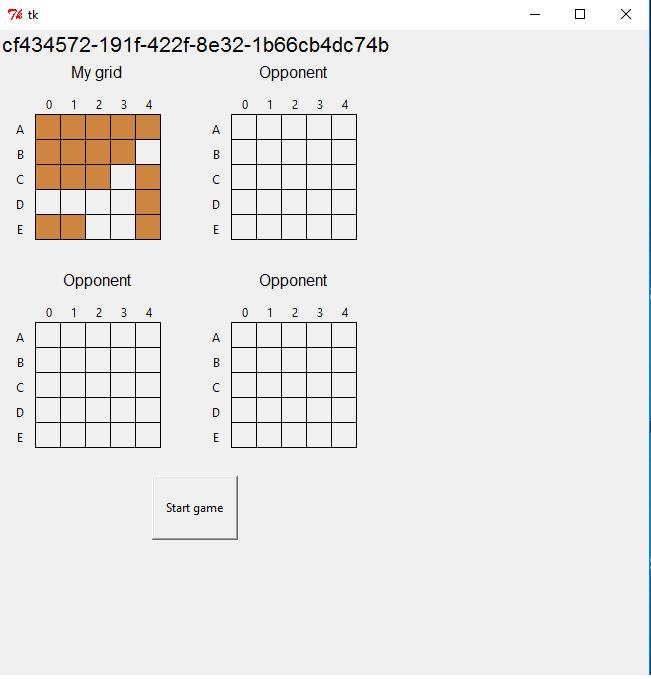
\includegraphics[width=0.8\textwidth]{WaitPage.png}
	\caption{Once ships are accepted, the user is directed to a wait-page. Master user has Start game button.}
	\label{fig:Waitpage}
\end{figure}

\begin{figure}[!hbt]
	\centering
	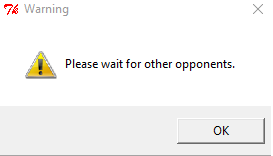
\includegraphics[width=0.8\textwidth]{WaitPlayers.png}
	\caption{If master starts game without other players, he is notified with a pop-up.}
	\label{fig:Waitplayers}
\end{figure}

\begin{figure}[!hbt]
	\centering
	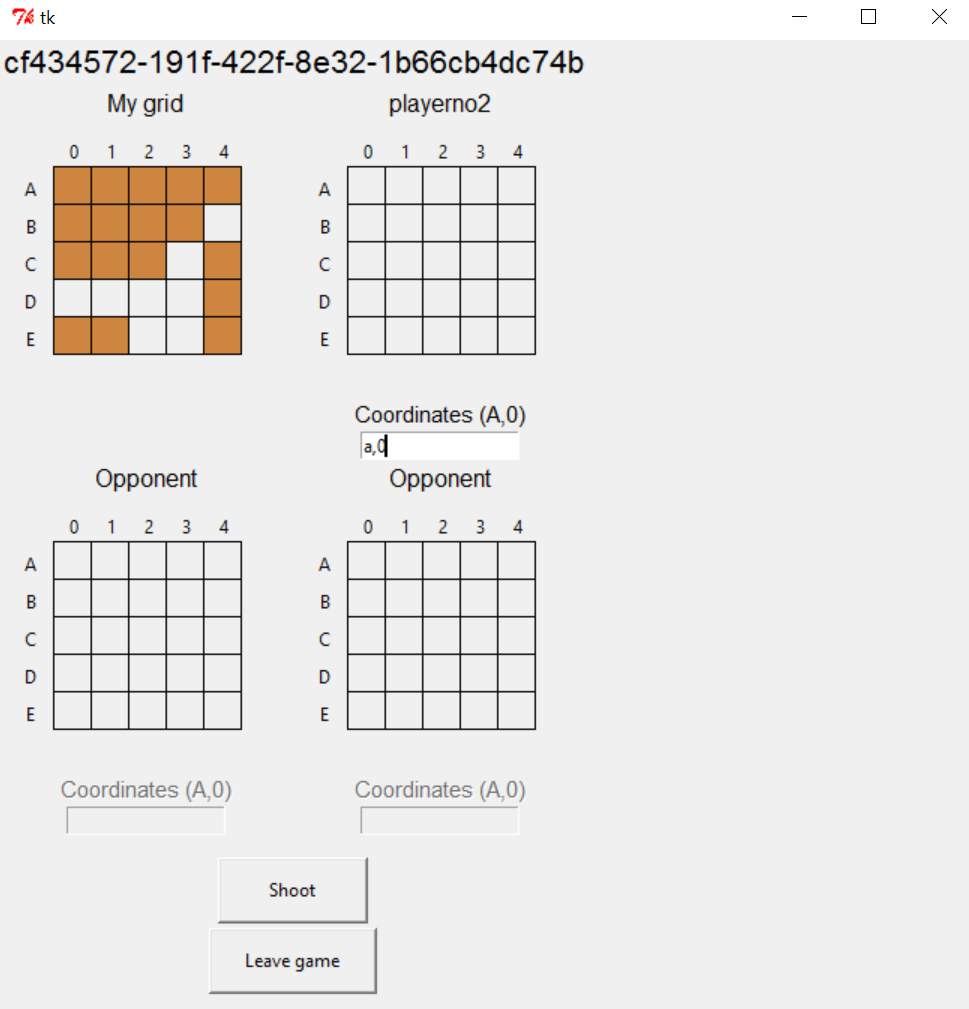
\includegraphics[width=0.8\textwidth]{GameOn.png}
	\caption{If the game has been started, the player whose turn it is can place their shots against the rest of the players whose names are displayed above the grids. If there are less than four player, excessive fields are disabled. Shoot button delivers the shots. Leave game button causes pop-up where user is asked whether they are sure they want to quit. If they are, then user leaves the game.}
	\label{fig:Gameon}
\end{figure}

\begin{figure}[!hbt]
	\centering
	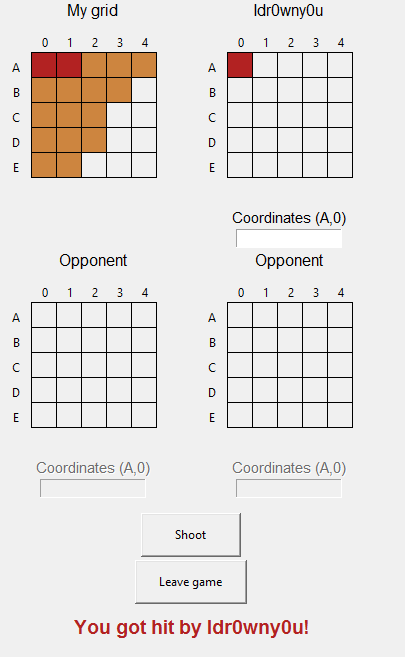
\includegraphics[width=0.8\textwidth]{GotHit.png}
	\caption{If a player is hit, the corresponding square is coloured red, missed shots are coloured as blue. Also a text is displayed for 3.5 seconds explaining who placed the scoring hit. Multiple hits to one square are allowed, but useless. Falsely placed hit is not accepted as a shot.}
	\label{fig:Gothit}
\end{figure}

\begin{figure}[!hbt]
	\centering
	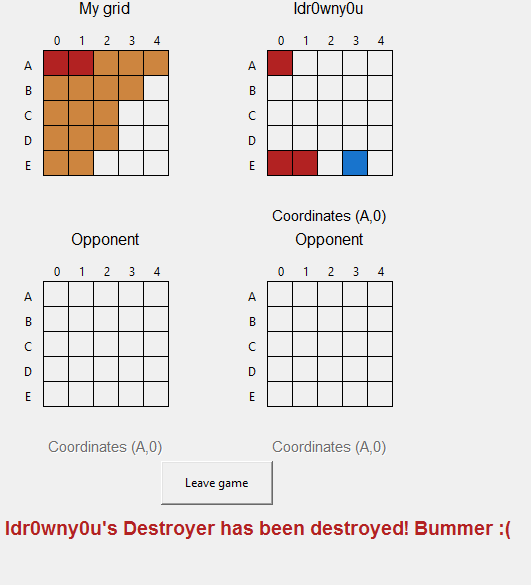
\includegraphics[width=0.8\textwidth]{ShipDown.png}
	\caption{If a player's ship is drowned, the message and placement of the ship is broadcast to everyone.}
	\label{fig:Shipdown}
\end{figure}

\begin{figure}[!hbt]
	\centering
	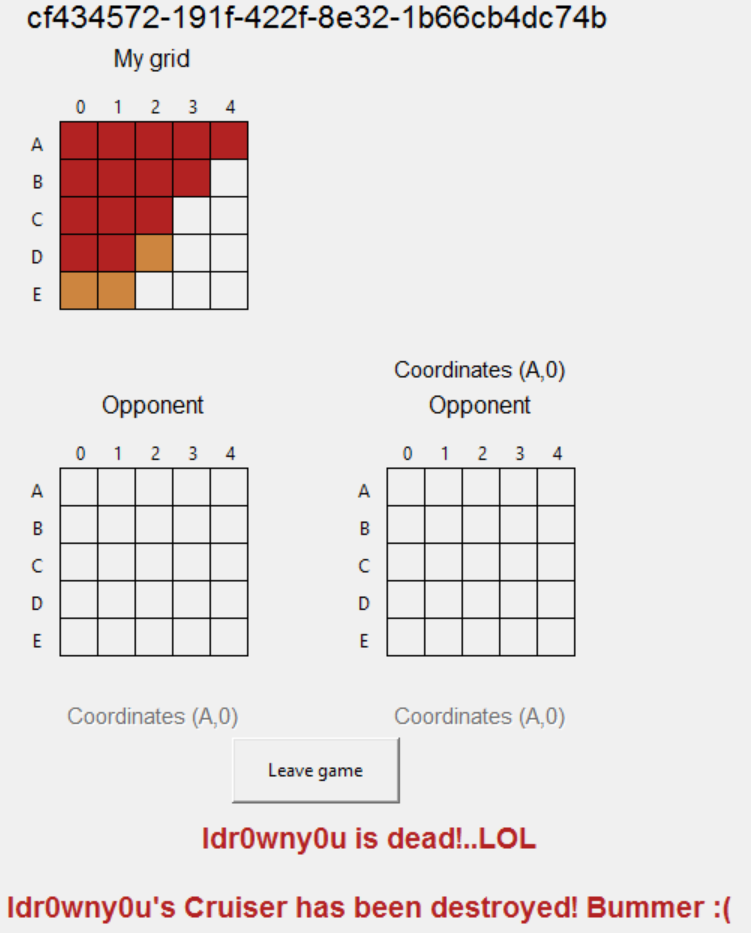
\includegraphics[width=0.9\textwidth]{PlayLost.png}
	\caption{If a player loses, it is broadcast to everyone in a polite manner, and their grid is made disabled to avoid confusion. If no more players remain, only Leave game is an option.}
	\label{fig:Playlost}
\end{figure}

\begin{figure}[!hbt]
	\centering
	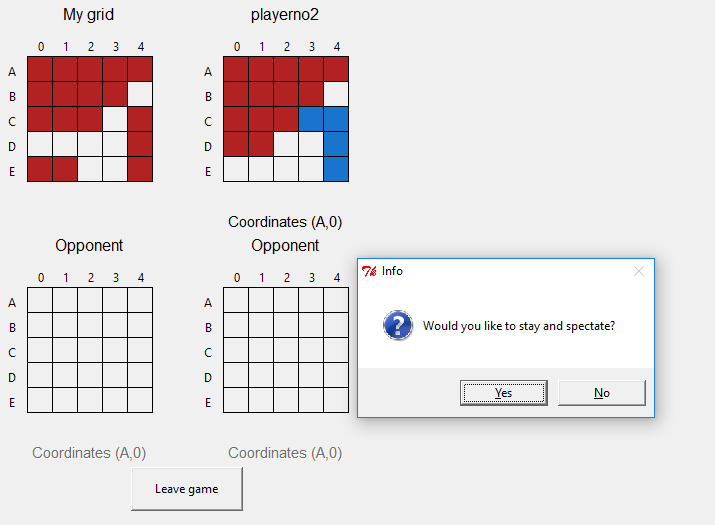
\includegraphics[width=0.9\textwidth]{LoserChoose.png}
	\caption{If a player loses, they are presented with a pop-up where they can either choose to remain spectating or leave the game to be directed to game choosing view.}
	\label{fig:LoserChoose}
\end{figure}

\begin{figure}[!hbt]
	\centering
	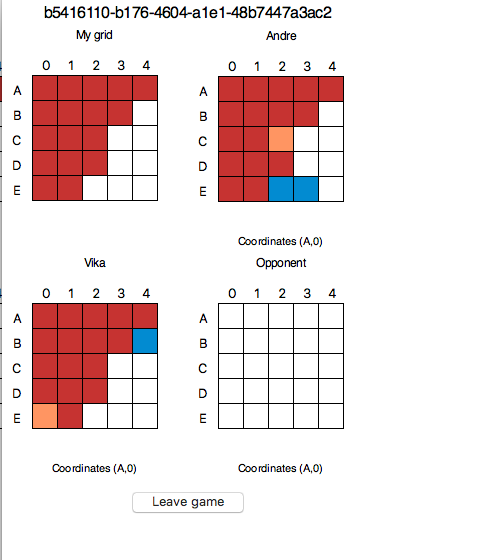
\includegraphics[width=0.8\textwidth]{SpectateInit.png}
	\caption{If a player chooses to stay and spectate the game then they see other players' ships (pale orange squares) and where others have been hit (red squares) or missed (blue squares). They see informative messages as before.}
	\label{fig:SpectateInit}
\end{figure}

\begin{figure}[!hbt]
	\centering
	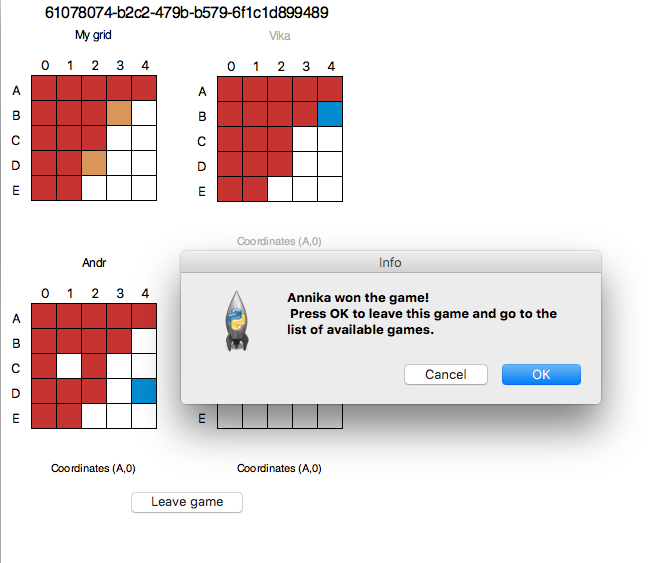
\includegraphics[width=0.9\textwidth]{Winner.png}
	\caption{When there is only one player left with some alive ships then everybody will get a notification about the winner.}
	\label{fig:Winner}
\end{figure}

\end{document}